\documentclass[english]{sareport}
% use the option peerreview for creating an anonymized version of your report
% E.g., \documentclass[english,peerreview]{sareport}

\usepackage[colorlinks, linkcolor=black, citecolor=black, urlcolor=black]{hyperref}
\usepackage{graphicx}
\usepackage{rotating}


% Set all authors, if your group counts 2, set third author empty \authorthree{}
% Set the groupname as well
\authorone{Monika Filipcikova (r0683254)}
\authortwo{Armin Halilovic(r0679689)}
\groupname{Filipcikova-Halilovic}

\academicyear{2016--2017}

\casename{Shared Internet Of Things Infrastructure Platform}
\phasenumber{1}
\phasename{Domain Analysis}


\begin{document}
\maketitle

\tableofcontents

\chapter{Domain analysis}\label{sec:domain}
\section{Domain models}
The domain model is shown in figure \ref{fig:domain_model}.

\begin{sidewaysfigure}[htp]
    \centering
    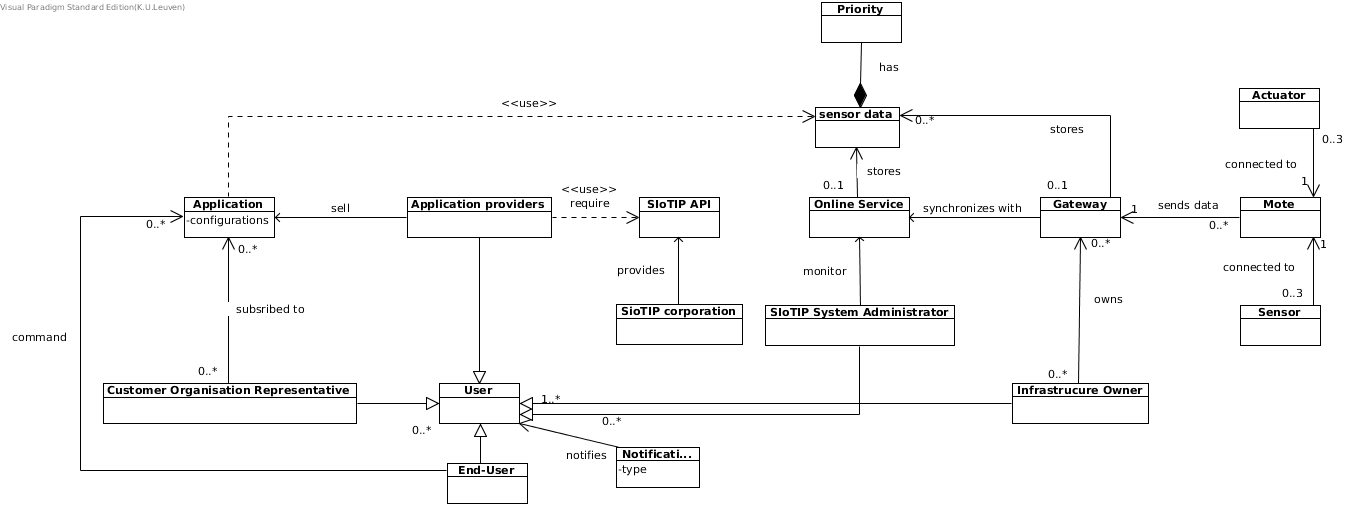
\includegraphics[width=1.05\textwidth]{Class_Diagram1.jpg}
    \caption{The domain model for the system.}\label{fig:domain_model}
\end{sidewaysfigure}

\section{Domain constraints}
In this section we provide additional domain constraints.

\begin{itemize}
    \item Gateways can to only run light-weight programs that are not too
          demanding in resources.
    \item The SIoTIP Online Service must be almost permamently available and sensor
          data is never lost or inconsistent.
    \item Core running inside SIoTIP must be able to interact with
          external applications and systems.
    \item Relaying information to the motes by the gateway is done by GET and PUT
          requests.
\end{itemize}

\newpage
\section{Glossary}
In this section, we provide a glossary of the most important terminology used
in this analysis.

\begin{itemize}
    \item \textbf{Application}: An application in the system is a program that
    uses sensors for a specific goal (e.g. fire detection). Customer organisations
    can subsribe to applications.
    \item \textbf{Application providers}: Application providers develop, upload,
    and maintain applications for the SIoTIP system.
    \item \textbf{Customer organisations}: Organisations that want to subscribe
    to applications. These organisations can subscribe to or unsubscribe from
    applications and get an overview of the invoices for their subscriptions.
    \item \textbf{Dashboard}: A dashboard is a collection of information which is
    available to a user. There are different dashboard for different type of users.
    \item \textbf{End-user}: End-users are the users that interact with deployed
    applications. They can issue commands to the application via a plethora of
    devices. For all end-users, the use of applications should simplify or
    automate their daily tasks.
    \item \textbf{Gateway}: A device which is connected to the Online Service
    and that has access to sensors and actuators. It can run some application
    logic and transmit data between the Online Service and the sensors/actuators.
    \item \textbf{Infrastructure owner}: This is someone who owns building(s),
    gateways, motes, sensors, and actuators. Owners are responsible for buying,
    installing, and maintaining hardware and the topology of their infrastructure.
    Owners can allocate installed hardware to specific customer organisations.
    \item \textbf{Mote}: A device that can host sensors and actuators. It connects
    these to the network and is used for communication between sensors/actuators
    and a gateway.
    \item \textbf{Notification}: A message that contains information about some
    event that occured in the system. Notifications have some priority. This
    influences how some notifications will be handled compared to others.
    \item \textbf{Online Service}: The online back-end which provides those
    services that are expected to generate the main revenue. Those services
    include the selling of hardware required for IoT infrastructures, and a
    platform where application providers and potential buyers can meet for a low price.
    \item \textbf{Replica}: definition
    \item \textbf{Sensor data}: Data about some sensor reading(s). Sensor
    data has some priority. This influences how some data will be handled
    compared to other data.
    \item \textbf{System}: "The system" is used to refer to the collection
    of entities that will be used by the SIoTIP corporation to render services.
    This includes the Online Service, gateways, motes, applications, etc.
    \item \textbf{System administrator}: System administrators monitor and
    manage the entire platform. They can view information about performance,
    running applications and sensors, shut applications down. These users are
    notified if alarming events threaten the platform.
    \item \textbf{User}: Someone who can log in and use parts of the system.
    Possibilities are system administrators, infrastructure owners, customer
    organisations, application providers, end-users.
\end{itemize}

\chapter{Functional requirements}\label{sec:functional}
\section{Use case model}

\begin{figure}[!htp]
    \centering
    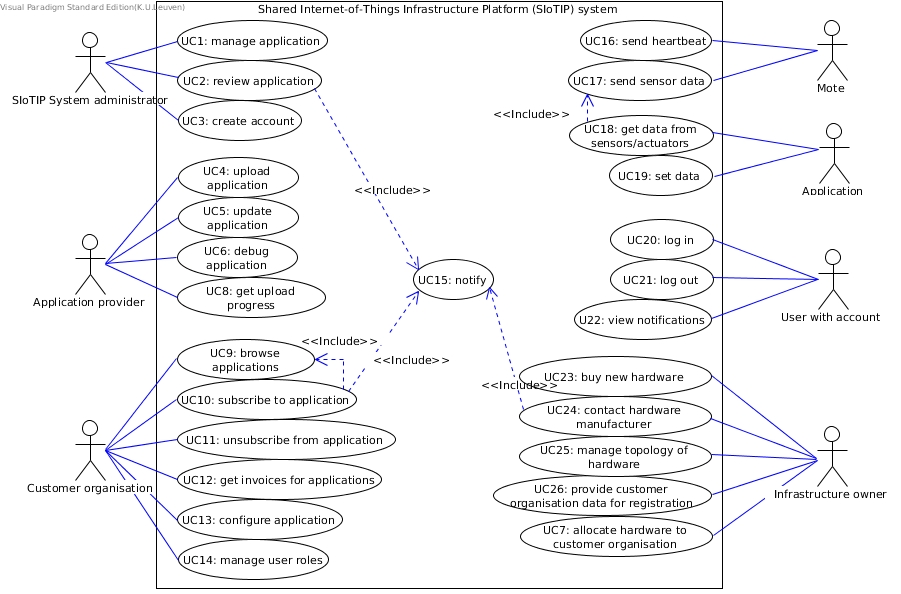
\includegraphics[width=1\textwidth]{Use_Case_Diagram1.jpg}
    \caption{Use case diagram for the system.}\label{fig:use_case_model}
\end{figure}

\section{Use case overview}\label{sec:uc_overview}

\paragraph{UCXXX: send data to gateway}
A mote sends data to a gateway.
\paragraph{UCXXX: upload application}
An appplication developers uploads an application to the Online Service.
\paragraph{UCXXX: get data from sensor}
An application requests to get data from a specific sensor.
\paragraph{UCXXX: search for applications}
A customer organisation representative searches for available applications they
could potentially subscribe to.
\paragraph{UCXXX: review application}
A SIoTIP system administrator reviews and approves or declines it.

\section{Detailed use cases}

\subsection{\emph{UCXXX}: Send sensor data}
\begin{itemize}
    \item \textbf{Name:} Send sensor data
    \item \textbf{Primary actor:} Mote
    \item \textbf{Secondary actors:} Sensor, Gateway
    \item \textbf{Interested parties:}
        \begin{itemize}
            \item \textit{Customer organisation:} pays for an application that uses this sensor.
            \item \textit{Infrastructure owner:} needs the sensor data for an application they set up.
            \item \textit{End-users:} use the sensor data in an application.
        \end{itemize}

    \item \textbf{Preconditions:}
        \begin{itemize}
            \item The mote has received data from a sensor connected to it.
            \item The mote is connected to a gateway.
        \end{itemize}

    \item \textbf{Postconditions:}
        \begin{itemize}
            \item The gateway has received and processed the sensor data.
            \item The Online Service has received the data and can process it.
        \end{itemize}

    \item \textbf{Main scenario:}
        \begin{enumerate}
           \item The mote sends the sensor data to the connected gateway.
           \item The gateway receives the data and if applicable, runs some application logic.
           \item The gateway collects data until a synchronisation point is reached.
                 At that point, the gateway sends the data to the Online Service.
        \end{enumerate}

    \item \textbf{Alternative scenarios:}
        \begin{enumerate}
            \item [3b.] The gateway determined that the data was important
                  (e.g. cause for alarm, notification, etc.) and sent the data
                  to the Online Service immediately instead of waiting for the
                  sycnhronisation point.
        \end{enumerate}

    \item \textbf{Remarks:}
        \begin{itemize}
            \item It is essential that the synchronisation protocol works
                  correctly in the presence of non-reliable network communication
                  so that there is no loss of data.
        \end{itemize}
\end{itemize}

\subsection{\emph{UCXXX}: Upload application}
\begin{itemize}
    \item \textbf{Name:} Upload application
    \item \textbf{Primary actor:} Application Developer
    \item \textbf{Secondary actor(s)}: SIotIP system
    \item \textbf{Interested parties:}
        \begin{itemize}
            \item \textit{Customers organisations:} want to subscribe the applications.
        \end{itemize}

    \item \textbf{Preconditions:}
        \begin{itemize}
            \item The application developer has access to his dashboard.
        \end{itemize}

    \item \textbf{Postconditions:}
        \begin{itemize}
            \item The application is uploaded into the Online Service.
            \item The application is available to customer organisations for subscription.
        \end{itemize}

    \item \textbf{Main scenario:}
    \begin{enumerate}
       \item The application developer logs in and opens his dashboard.
       \item The system provides the ability to upload new application.
       \item The application developer uploads application.
       \item The system check application and  initiates a number of automated tests.
       \item The application developer follows  the  progress  and  results  
             of these tests via application provider dashboard.
       \item The application successfully passes all tests.
       \item The system makes the application available for the customers organisations.
       \item The system send a notification to the application developer.
    \end{enumerate}

    \item \textbf{Alternative scenarios:}
    \begin{enumerate}
        \item [4b.] The system can not load application and send error 
                    to the application developer.
        \item [7b.] The system interrupt loading of the application, 
                    because of potential memory leak.
        \item [8b.] The SIoTIP administrator performs a secondary review and decides whether to accept
                    or reject the application.
    \end{enumerate}

    \item \textbf{Remarks:}
        \begin{itemize}
            \item First remark
        \end{itemize}
\end{itemize}

\subsection{\emph{UCXXX}: Get data from sensor}
\begin{itemize}
    \item \textbf{Name:} Get data from sensor
    \item \textbf{Primary actor:} Application
    \item \textbf{Secondary actor(s)}: Online Service, Gateway, Mote
    \item \textbf{Interested parties:}
        \begin{itemize}
            \item \textit{End-user:} wants to get information from sensors
        \end{itemize}

    \item \textbf{Preconditions:}
        \begin{itemize}
            \item The application is uploaded in Online Service.
            \item A connection between Online Service and Getway is established.
        \end{itemize}

    \item \textbf{Postconditions:}
        \begin{itemize}
            \item The application received data from sensor.
        \end{itemize}

    \item \textbf{Main scenario:}
    \begin{enumerate}
       \item The application send request to Online Service.
       \item The Online service communicate with the Gateway.
       \item The Gateway relay information to the mote by sending request.
       \item The mote send data to Online Service (include:send sensor data (UCXX))
       \item The Online Service send data to the application.
    \end{enumerate}

    \item \textbf{Alternative scenarios:}
    \begin{enumerate}
        \item [5b.] 5b. The application does not receive any data within 2s. 
                    It will retry the request 2 more times.
    \end{enumerate}

    \item \textbf{Remarks:}
        \begin{itemize}
            \item First remark
        \end{itemize}
\end{itemize}

\subsection{\emph{UCXXX}: Search for applications}
\begin{itemize}
    \item \textbf{Name:} Search for applications
    \item \textbf{Primary actor:} Customer orgranisation
    \item \textbf{Secondary actor(s)}: secondary actor(s)
    \item \textbf{Interested parties:}
        \begin{itemize}
            \item \textit{Name of interested party:} reason why party is interested
        \end{itemize}

    \item \textbf{Preconditions:}
        \begin{itemize}
            \item The primary actor is authenticated.
            \item The customer organisation wants to install new application.
        \end{itemize}

    \item \textbf{Postconditions:}
        \begin{itemize}
            \item First postcondition.
            \item Second postcondition.
        \end{itemize}

    \item \textbf{Main scenario:}
    \begin{enumerate}
       \item Step 1
       \item Step 2
       \item Step 3
       \item \ldots
    \end{enumerate}

    \item \textbf{Alternative scenarios:}
    \begin{enumerate}
        \item [3b.] Alternative at step 3
    \end{enumerate}

    \item \textbf{Remarks:}
        \begin{itemize}
            \item First remark
        \end{itemize}
\end{itemize}

\subsection{\emph{UCXXX}: Review application}
\begin{itemize}
    \item \textbf{Name:} Review application
    \item \textbf{Primary actor:} SIoTIP System Administrator
    \item \textbf{Secondary actor(s)}:
    \item \textbf{Interested parties:}
        \begin{itemize}
            \item \textit{Application developers:} want to add their application to the system
        \end{itemize}

    \item \textbf{Preconditions:}
        \begin{itemize}
            \item The system administrator is authenticated.
            \item The application needs to be reviewed by a system administrator.
        \end{itemize}

    \item \textbf{Postconditions:}
        \begin{itemize}
            \item The system adminstrator accepts or declines the application.
            \item The application developers have been notified of this event.
        \end{itemize}

    \item \textbf{Main scenario:}
        \begin{enumerate}
            \item The system administrator navigates to the applications component on their
                  dashboard and selects the application that needs to be reviewed.
            \item The system administrator reviews the application's functionality and
                  log history, and the message history with the developers.
            \item The system administrator indicates he wants to accept the application.
            \item The system logs this event and makes the application available to
                  customer ogranisations.
            \item The system notifies the application developers.
        \end{enumerate}

    \item \textbf{Alternative scenarios:}
        \begin{enumerate}
            \item [3b.] The system administrator indicates he wants decline to the application
                  and is prompted by the system to fill in the reason for this. The
                  application will thus not become available to customer organisations.
            \item [3c.] The system administrator indicates he wants communicate
                  with the developers before making a decision. Afterwards, return to
                  step 2.
        \end{enumerate}

    \item \textbf{Remarks:}
        \begin{itemize}
            \item When an application first gets uploaded to the system, it needs to be
                  reviewed and accepted by a system administrator. This will prevent
                  the available apps to be flooded with apps of very poor quality
                  or apps that are copies of other apps.
            \item If at some point in the future, automated testing for an app fails,
                  the app will need to be reviewed again before it can be made
                  available again.
        \end{itemize}
\end{itemize}

\chapter{Non-functional requirements}\label{sec:non-functional}
In this section, we model the non-functional requirements for the system in the
form of \emph{quality attribute scenarios}. We provide for each type
(availability, performance and modifiability) one requirement.

\section{Availability}
\subsection{\emph{Av1}: Unusable database}
A database in the system cannot be used anymore. This could happen because of
corrupted disks, power outages, too many requests coming into the database
server, network failures, natural physical disasters, etc. A different database
will be used while this one is unusable.

\begin{itemize}
    \item \textbf{Source:} Database server
    \item \textbf{Stimulus:}
        \begin{itemize}
            \item The database crashed.
            \item The database does not respond to requests.
            \item The database does not respond to requests within reasonable time.
            \item The database returns invalid data or responses.
        \end{itemize}

    \item \textbf{Artifact:} Persistent storage
    \item \textbf{Environment:} Normal operation
    \item \textbf{Response:}
        \begin{itemize}
            \item Use a working replica until the database can be used again.
            \item Log the fault.
            \item If the problem with the database cannot be fixed automatically
                  (e.g. by an automatic restart and resynchronisation), send
                  a technician if it is possible for them to fix the problem
                  (e.g. replace corrupted disks). Otherwise (e.g. power outages,
                  natural physical disasters), send a notification
                  of high priority to SIoTIP system administrators.
        \end{itemize}

    \item \textbf{Response measure:}
        \begin{itemize}
            \item If a database becomes unusable, this should be detected
                  within 3s of the system trying to use the database.
            \item When the system detects that a database is unusable,
                  a working replica should be used within 5s.
            \item If a database is unusable because of a system crash or user error,
                  the database should restart and start its boot procedure within 5s.
            \item If a database is unusable because of corrupted disks, a technician
                  should replace the disk within 30 min.
        \end{itemize}
\end{itemize}

\subsection{\emph{Av2}: Broken sensor}
A sensor breaks. The infrastructure owner is notified and if possible, another
sensor is used for the responsibility that the broken one was fulfilling.

\begin{itemize}
    \item \textbf{Source:} Sensor
    \item \textbf{Stimulus:}
        \begin{itemize}
            \item No data can be received anymore from the sensor.
            \item The sensor stopped sending regular updates.
            \item The sensor sends invalid/corrupted data.
            \item The sensor disappeared from the heartbeats of the mote it
                  is connected to.
        \end{itemize}

    \item \textbf{Artifact:} Communication channel between sensor and gateway
    \item \textbf{Environment:} Normal operation
    \item \textbf{Response:}
        \begin{itemize}
            \item The gateway uses another sensor to be used for
                  the same responsibility as the broken one.
            \item Log the fault and notify the infrastructure owner.
        \end{itemize}

    \item \textbf{Response measure:}
        \begin{itemize}
            \item When a sensor breaks, this is detected within 2s.
            \item If there is another sensor that can fulfill the same responsibility
                  as the broken one, it should be chosen within 2s.
        \end{itemize}
\end{itemize}

\section{Performance}
\subsection{\emph{P1}: Application requests under peak load}
An application sends requests to the Online Service while the system is under
peak load. These requests could be for getting data from a specific
sensor, for configuring application settings, etc.
These request should be processed in a timely manner.

\begin{itemize}
    \item \textbf{Source:} Application
    \item \textbf{Stimulus:}
        \begin{itemize}
            \item An application sends a request to the Online Service.
        \end{itemize}

    \item \textbf{Artifact:} The whole system
    \item \textbf{Environment:} Under peak load
    \item \textbf{Response:}
        \begin{itemize}
            \item When a request comes into the system, core work necessary
                  to generate a reply is done first. Other work of less importance
                  (e.g. sending emails, generating low-priority notifications, etc.)
                  is scheduled to be done later.
            \item Load balancing is used to divide the requests over
                  available servers.
            \item Servers that are closest to source of the request are chosen
                  over servers that are farther away to minimize network delay.
        \end{itemize}

    \item \textbf{Response measure:}
        \begin{itemize}
            \item Applications get a response within 3s.
        \end{itemize}
\end{itemize}

\subsection{\emph{P2}: Mote data to application delay}
When a mote sends data to an application, that data reaches its
destination in a bounded time. This bound is determined by the priority
of the data. The possible priorities are low, medium, and high.
These priorities can be set by an infrastructure owner.

\begin{itemize}
    \item \textbf{Source:} Mote
    \item \textbf{Stimulus:}
        \begin{itemize}
            \item A mote sends data to an application.
        \end{itemize}

    \item \textbf{Artifact:} The whole system
    \item \textbf{Environment:} Normal operation
    \item \textbf{Response:}
        \begin{itemize}
            \item The data is always sent to the next node before other extra
                  work is done. For example, other work could be logging
                  or sending notifications.
        \end{itemize}

    \item \textbf{Response measure:}
        \begin{itemize}
            \item If the data priority is low, the data reaches the application
                  within 60s.
            \item If the data priority is medium, the data reaches the application
                  within 10s.
            \item If the data priority is high, the data reaches the application
                  within 1s.
        \end{itemize}
\end{itemize}

\section{Modifiability}
\subsection{\emph{M1}: Add a new type of sensor}
The SIoTIP corporation wishes to provide a new type of sensor to customers.

\begin{itemize}
    \item \textbf{Source:} SIoTIP developer
    \item \textbf{Stimulus:}
        \begin{itemize}
            \item Developers add a new type of sensor to the system
        \end{itemize}

    \item \textbf{Artifact:} System codebase and database.
    \item \textbf{Environment:} Normal operation, during a development iteration
    \item \textbf{Response:}
        \begin{itemize}
            \item The software on motes and gateways must be updated so that
                  the new sensor can be read, calibrated and configured.
            \item Components in the system responsible for storage of sensor readings
                  must be updated to save the readings of the new sensor correctly.
            \item UI components must be updated so that the readings of the
                  new sensor can be displayed correctly.
            \item This modification does not affect the way data is communicated
                  whithin components of the system.
            \item Infrastructure owners can choose when the update will happen.
                  The motes and gateways must be updated before the new
                  typ of sensor can be ordered.
            \item The updates to the UI components and storage components can
                  be deployed at run time.
                  There is no need to destroy any login sessions for this, since the
                  sensor will not be in use at that time yet.
        \end{itemize}

    \item \textbf{Response measure:}
        \begin{itemize}
            \item This modification is finished within 5 man months of development time.
            \item The deployment of the modifications to the UI components and storage
                  components is finished within 10 minutes.
        \end{itemize}
\end{itemize}

\subsection{\emph{M2}: Changes to UI components or new UI components}
Developers want to add or edit components that make up the UI.
For example, they want to improve components that are reused in dashboards.

\begin{itemize}
    \item \textbf{Source:} SIoTIP developers
    \item \textbf{Stimulus:}
        \begin{itemize}
            \item Developers add a UI component.
            \item Developers edit a UI component.
        \end{itemize}

    \item \textbf{Artifact:} User interface and platform.
    \item \textbf{Environment:} Normal operation, during a development iteration
    \item \textbf{Response:}
        \begin{itemize}
            \item Users are not able to use the system during the deployment
                  of the changes. All users that are logged in at the time
                  the deployment starts will be logged out first.
            \item All users are notified in advance of incoming downtime.
            \item The update does not affect currently ongoing activity in
                  the system.
            \item The update only affects the subsystem responsible for the UI.
        \end{itemize}

    \item \textbf{Response measure:}
        \begin{itemize}
            \item The deployment of the new UI components is finished within 30 minutes.
                  Users can log in again immediately after the deployment is finished.
        \end{itemize}
\end{itemize}

\section{Usability}
\subsection{\emph{U1}: System administrator reviews application}
Before an application can be published or when its automated tests
fail, it needs to be reviewed by a SIoTIP system administrator.

\begin{itemize}
    \item \textbf{Source:} SIoTIP system administrator
    \item \textbf{Stimulus:}
        \begin{itemize}
            \item The system administrator wants to review the application
                  and/or test logs quickly.
            \item The system administrator wants to contact the application
                  provider.
        \end{itemize}
    \item \textbf{Artifact:} System administrator dashboard
    \item \textbf{Environment:} At normal operation
    \item \textbf{Response:}
        \begin{itemize}
            \item The system administrator dashboard is built up using clear
                  components which contain informations about different
                  elements of the system. One such component displays applications
                  that are waiting for a review.
            \item The application review page contains a component that
                  describes the application's functionality. There are clear
                  buttons to accept or decline the application. There is a
                  button to open the application.
            \item Optionally, the application review contains a component which
                  displays images  of the application from an infrastructure
                  owner's point of view.
            \item There is a component which displays the log history of the application.
            \item There is a component for communication with the application provider.
        \end{itemize}

    \item \textbf{Response measure:}
        \begin{itemize}
            \item All actions for reviewing the application, accepting or
                  declining the application, reading the application's log history,
                  and contacting the application provider are possible within 5 clicks.
        \end{itemize}
\end{itemize}

\subsection{\emph{U2}: User wants to learn to use the system}
A user wants work with the system efficiently. He wants to learn to use the system
by reading guides for tasks or by searching for specific infomation quickly.
An easy to use help system is put in place for this.

\begin{itemize}
    \item \textbf{Source:} User
    \item \textbf{Stimulus:}
        \begin{itemize}
            \item The user wants to learn system features.
            \item The user wants to feel comfortable with his dashboard.
        \end{itemize}

    \item \textbf{Artifact:} Help subsystem, UI components
    \item \textbf{Environment:} At normal operation
    \item \textbf{Response:}
        \begin{itemize}
            \item The user uses the help system to learn about the functionality
                  every page. When this help system is used, it displays
                  key information about the page the user is currently
                  on.
            \item The help system contains a search form so the user can learn about
                  anything they want that is relevant to their dashboard.
            \item For each task a specific type user can perform, the help system
                  contains a guide that explains the process step by step.
            \item The user's dashboard consists of clear UI components that
                  provide information about different elements of the system.
            \item All forms have clear error notifications. The user is navigated the right way
                  when he does something wrong.
        \end{itemize}

    \item \textbf{Response measure:}
        \begin{itemize}
            \item Anything the user would want to know about relevant to the system
                  can be learned within 5 clicks.
        \end{itemize}
\end{itemize}


\end{document}
